\documentclass{article}
\usepackage[letterpaper, left=2.5cm, right=2.5cm, top=2.5cm, bottom=2.5cm]{geometry}
\usepackage{graphicx}
\usepackage{epstopdf}
\usepackage{enumitem}
\usepackage{fge}

\setdescription{leftmargin=\parindent, labelindent=\parindent}

\begin{document}

\title{PAL Compiler Documentation }
\date{\today}
\author{Chris Pavlicek, Connor Moreside, Mike Armstrong, and Steve Jahns}
\maketitle

% From checkpoint 1 spec:
%
% Documentation
%
% Your documentation should describe what your group has done on the
% project. This does not mean that you should reiterate class notes; I want to
% know what is different about your group. Some things you may want to discuss
% include: handling of lexical units, syntax error reporting strategies, syntax
% error recovery (if any) , problems encountered and their solutions, etc.
% When writing, remember who is going to read it—skip the preli minaries
% and get to the point. There is a page limit of 12 double-spaced pages,
% not in cluding diagrams.

\section*{Overview}

\begin{figure}[h!]
\centering 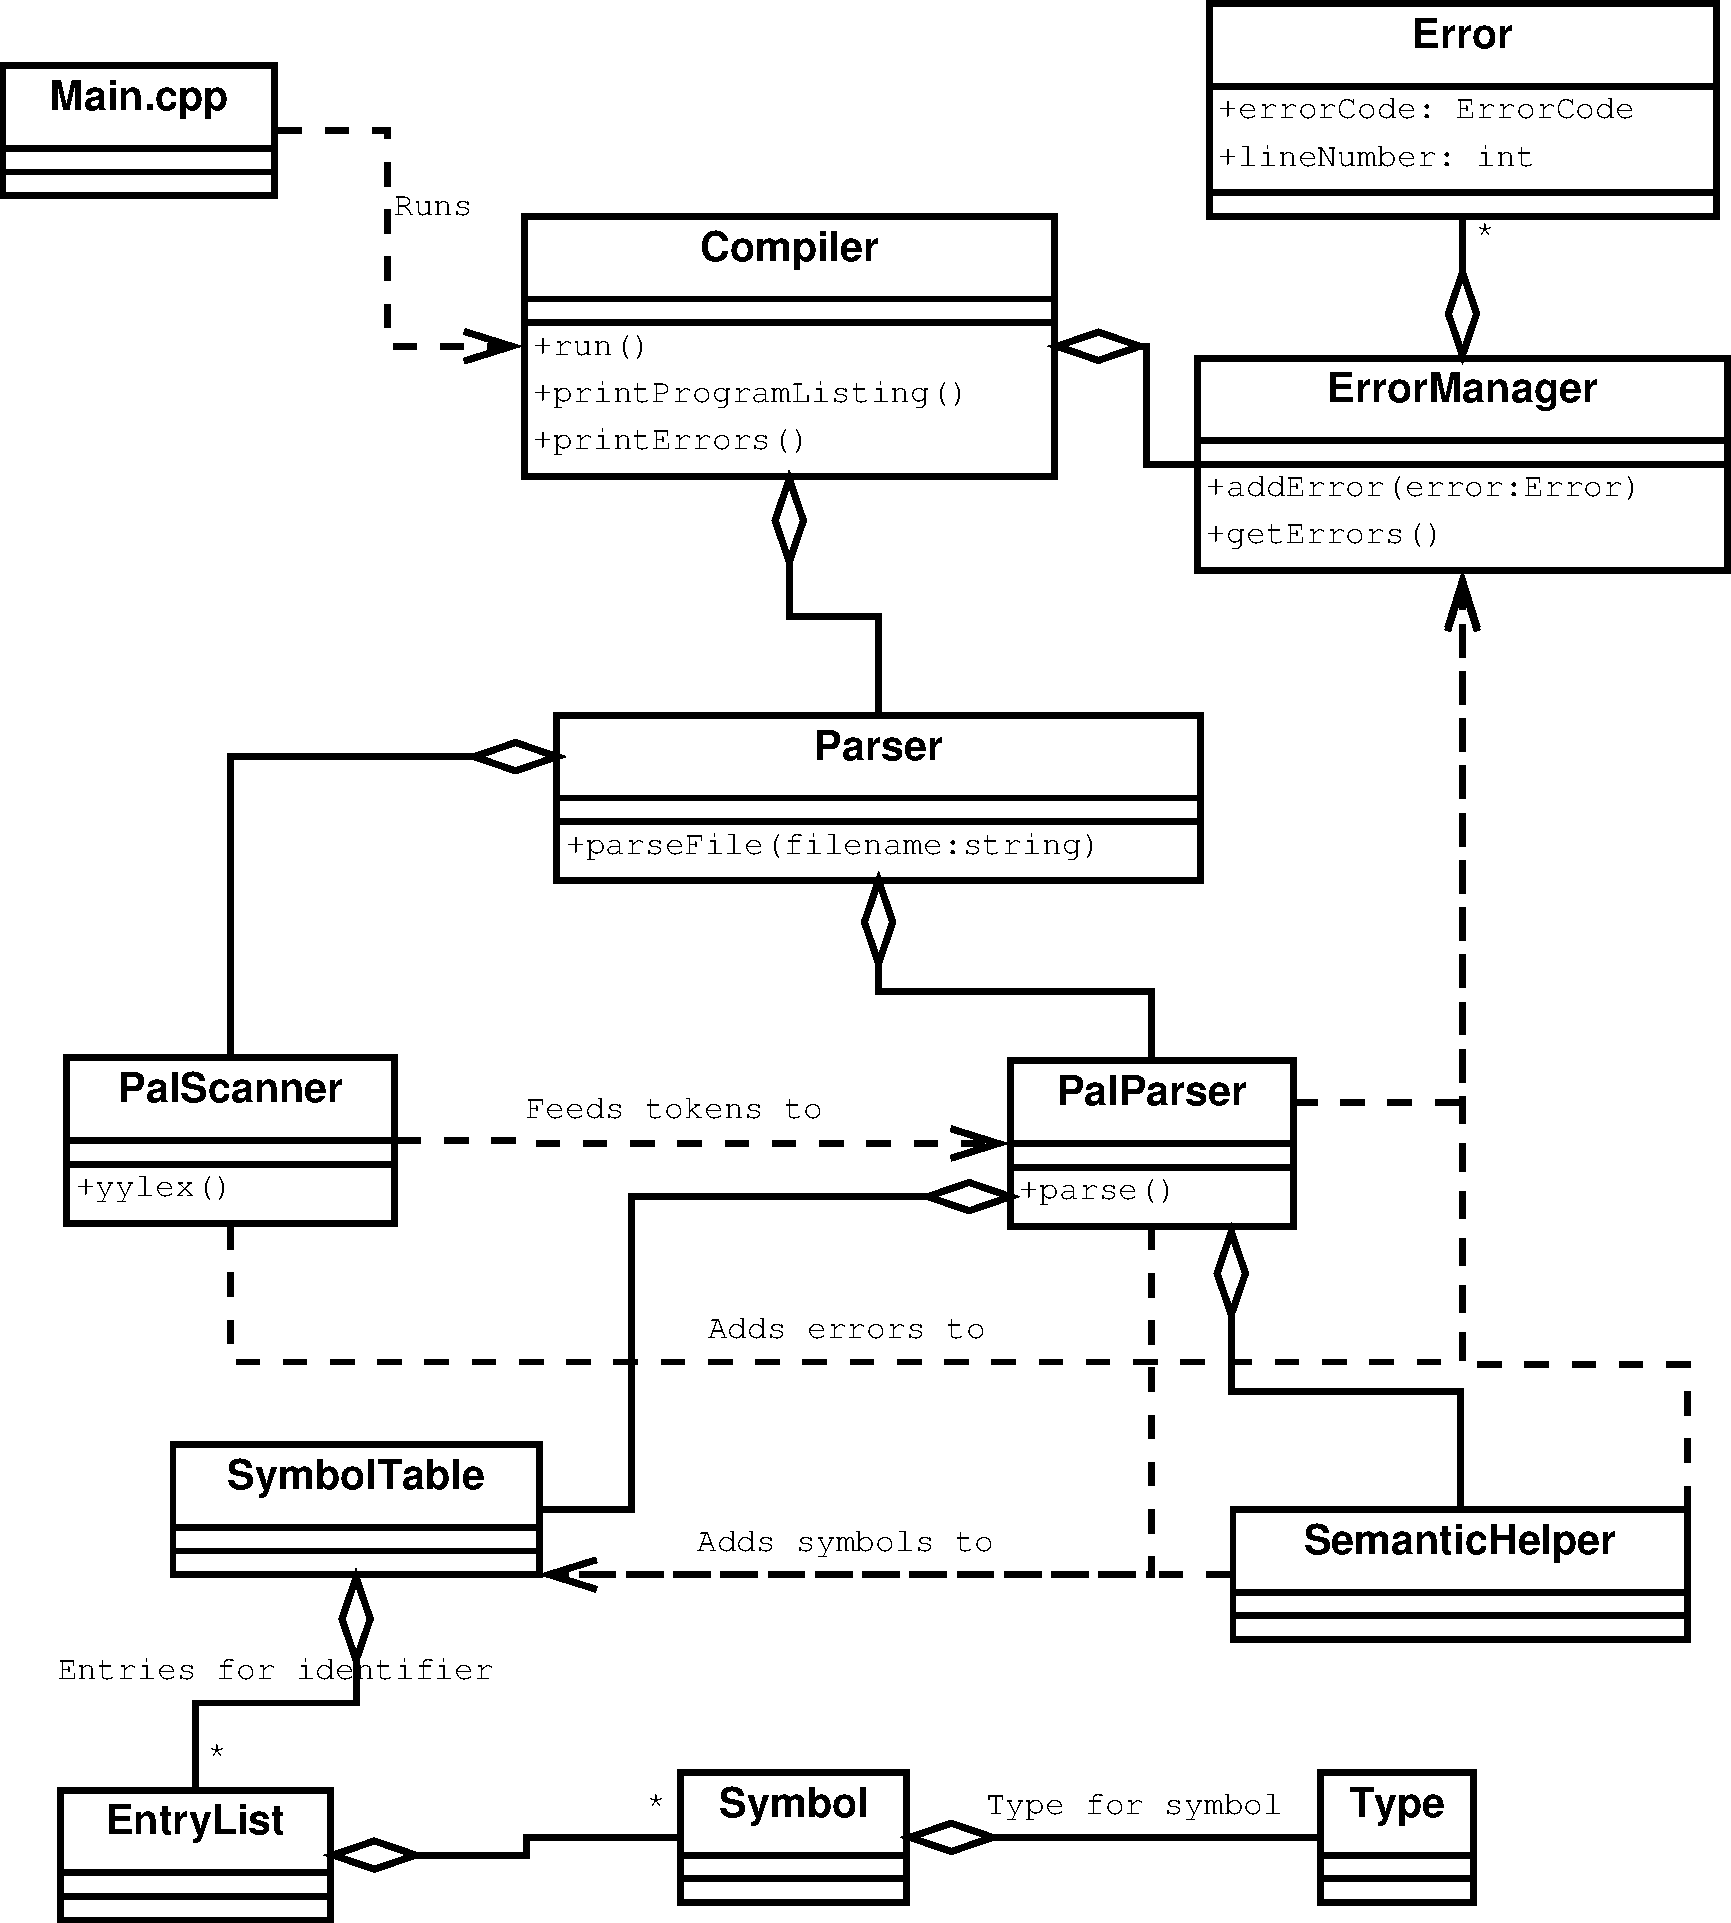
\includegraphics[width=13cm]{uml.pdf}
\caption{General structure of the compiler's parsing and semantic analysis components.}
\end{figure}

At this stage, our compiler source consists of 10 classes. The \texttt{Compiler} class is instantiated by 
the program's \texttt{main()} function, and ran with the program's given command line arguments. 

The \texttt{Compiler} class creates an \texttt{ErrorManager}
class which tracks errors as they are detected while parsing the file. It passes the \texttt{ErrorManager}
to the \texttt{Parser} class when it is constructed.

The \texttt{Parser} class is a wrapper for the \texttt{flex} and \texttt{bison}
generated \texttt{PalScanner} and \texttt{PalParser} classes, from the
\texttt{pal.lex} and \texttt{pal.y} sources, respectively. \texttt{Parser}
parses a file with \texttt{parseFile(fileName)}, which creates a
\texttt{PalScanner} and \texttt{PalParser} where the scanner runs through
the file and feeds the parser with a stream of tokens.  The scanner and
parser are given access to the common \texttt{ErrorManager}, and when they
encounter errors during lexical and syntactical analysis, they create new
\texttt{Error} objects with the appropriate error code and line number and
give them to the \texttt{ErrorManager}.

Semantic checking is primarily completed by the \texttt{SemanticHelper} class and of course
the symbol table (\texttt{SymbolTable}). We currently have a monolithic symbol class (\texttt{Symbol}),
which can represent the various identifier constructs available in PAL.

When parsing and semantic checking have finished, the \texttt{Compiler} takes the errors accumulated by
the \texttt{ErrorManager} and either displays them inline with the program
listing, or all errors in order of appearance without the program listing if 
\texttt{pal} was invoked with the \texttt{-n} option.

	% Overall design
	% Outline of classes + dependencies

\section*{Lexical Analysis}

Our lexical analyser is generated by GNU Flex from the source in \texttt{./src/pal.lex}, which
is bundled into the \texttt{PalScanner} class. It is capable of recognizing the following
errors at the lexical level:

\begin{description}
  \item[Unclosed Comment]
	  If a comment is started with \texttt{\{} but is not followed by a
	  \texttt{\}} later in the file, the scanner will report an error.  In
	  our scanner, the comment rule will match to the end of the file in
	  this situation, so unfortunately no more analysis of the file is
	  possible at this point.
	  % TODO should we consider backtracking to the next line somehow?

  \item[Unexpected Comment End]
	  If the scanner encounters a \texttt{\}} when it is not in a comment,
	  it will report an error. Otherwise, the extra brace is ignored and analysis 
	  continues in an attempt to find more errors in the file.

  \item[Multi-line String Literal]
	  % TODO make sure this is actually implemented!
	  In the PAL language, a string literal cannot span multiple lines, so 
	  if the scanner encounters a string literal that extends beyond the next
	  newline, it will report an error that indicates the start and finish line
	  of the illegal multi-line string. It will still return a \texttt{STRING\_LITERAL}
	  token, and continue analysis to try and find more errors.

  \item[Invalid Character or Escaped Character in String]
	  The scanner will report an invalid character/escaped character in a string
	  literal if it contains either of the following:
	  \begin{itemize}
		  \item a \texttt{\textbackslash} that is not followed by a 
			  \texttt{'}, \texttt{n}, or \texttt{t}
		  \item a \texttt{\textbackslash} at the end of the string, that
			  is not preceded by another \texttt{\textbackslash}
	  \end{itemize}

	  % TODO would be cool if it actually printed the invalid character!

	% TODO \ at end of string? what kind of error? test!?

  \item[Invalid Identifier]
	  Valid PAL identifiers start with at least one letter, followed by any number
	  of letters or numbers. Identifiers that start with numbers will be reported
	  as an error. 
	% TODO can we detect other invalid identifiers?

  \item[Invalid character]
	  If the scanner detects an unknown character, such as \texttt{!} or
   \texttt{\#}, it returns an error indicating that an unrecognized
   character was found. It easily recovers from this error and
   continues on. 


\end{description}

\section*{Syntax Analysis}
Our syntax analyzer is generated by GNU Bison from the source in \texttt{./src/pal.ly}, which
is bundled into the \texttt{PalScanner} class. It is capable of recognizing the following
errors at the syntax level:

\begin{description}
  \item[Program Declarations]
	The compiler detects faults in the declaration. If it is missing a program
	will not compile. Errors will be outputted for the following cases:
		\begin{itemize}
			\item If the semicolon is missing
			\item If one or both arguments are missing
			\item If the program is missing a closing parentheses,
			starting, or both.
			\item If there is an invalid program name
		\end{itemize}
\item[Variable, Constant or Type Declarations]
	If a variable, constant or type is incorrectly declared, the compiler will
	catch the following errors:
		\begin{itemize}
			\item If an improper type of assignment is used. IE. 
			constant is declared using :, instead of = an appropriate
			error message will be emitted for each type.
			\item Improper variable names, only variables starting with
			a letter, and containing letters and numbers after are valid.
		\end{itemize}
		
\item[Enumerations]
	If an enumeration is incorrectly defined an error will be produced.
\item[Arrays]
	Arrays which are declared incorrectly, either by defining the set wrong, 
	or by specifying an invalid type will produce a specific error.
\item[Functions]	
	Functions will be checked for proper formatting if a function is invalid 
	an appropriate error will be emitted. Functions are required to have 
	return types, enclosing parameters and a ending semicolon. Each function 
	is required to have variables declared before the begin statement and required
	to be have a begin and end statement.
	
\item[Procedures]
	Procedures are declared in a similar fashion as functions, and have the same
	error checking except that they don't have a return value and are ended by 
	a period instead of a semicolon. 

\item[Expressions]
	Expressions will checked for proper structure. If a symbol is missing,
	semicolon or any part it will be discarded and return an error. 
	
\item[Recovery Strategies]
	Try to catch errors as early as possible by defining strict cases that are
	simple to implement but are common user errors. Errors which are not defined
	are given a generic error output, using the built in error within bison.

	% TODO
	% handling of lexical units
	% syntax error reporting
	% recovery strategies
\end{description}

\section*{Semantic Analysis}
Semantic analysis first begins within the bison grammar file, \texttt{./src/pal.y}. 

There exists two main classes for encapsulating information regarding the type of a particular symbol,
and the symbol itself.

Firstly, we have the monolithic \texttt{Symbol} class, which is responsible for capturing important information regarding any
given identifier in a PAL program, including variable declarations, function declarations, enums,
and so forth.

And secondly, there is a class which encapsulates information regarding types in PAL, which was aptly named \texttt{Type}.
This class is responsible for holding information about any type that can be declared in a valid PAL program. It has fields 
for records, functions, primitive types...

We make use of a class called \texttt{SemanticHelper} to encapsulate some of the semantic analysis 
functionality in order to keep the grammar file relatively clean.

The \texttt{SemanticHelper} performs the following functions:

\begin{description}
	
\item[Pre-Populate Symbol Table]
	There exists a function which populates the symbol table with various pre-defined types,
	functions, constants, etc...
	
\item[Perform Type Comparisons]
	Since the \texttt{SemanticHelper} class has a reference to the symbol table, it is able to
	perform a type comparison between two separate constructs, such as variables, constants, etc...
	
\item[Add New Types To Symbol Table]
	When a new type is encountered in a PAL program, the \texttt{SemanticHelper} is responsible for creating
	a new \texttt{Symbol} and corresponding \texttt{Type}. This information is then added into the symbol table.
	
\item[Retrieve Type After Expression Evaluation]
	During the evaluation of certain statements, the final type of the an operations must be determined in order
	to determine type compatibility. The \texttt{SemanticHelper} is responsible for this.
	
\item [Retrieve Primitive Types]
	Pre-defined \'raw\' types such as boolean, integer, real, etc... are retrieved using this class.

\end{description}
	
%% TODO
% Talk about construction of Symbol Table; functions, data structures, etc...

The symbol table is contained in the \texttt{SymbolTable} class. Our symbol table was built around the C++ pre-defined
\texttt{unordered\_map}. This was quite nice since we did not have to define our own hash map implementation, thus
greatly reducing the chances of bugs due to improper implementation. 

Within a bucket of the top level hash map, there is a class called \texttt{EntryList}. It is essentially a vector containing the definitions of symbols at various lexical levels. The symbol table's methods handle the different definitions at various
levels with ease.

The Symbol table contains the following functionality:

\begin{description}
	
\item[Adding Symbol]

\item[Finding The Definition Of A Symbol]

\item[Retrieving A Symbol]

\item[Retrieving The Current Lexical Level]

\item[Incrementing The Lexical Level]

\item[Decrementing The Lexical Level]
	
\end{description}

As you can see, the \texttt{SymbolTable} and \texttt{SemanticHelper} classes work very closely together
in order to perform semantic checking.

\section*{Our Failed Abstract Syntax Tree}

When beginning Checkpoint 2, we started to create an AST structure so we could cleanly separate semantic analysis 
and code generation functionality from the grammar file. Initially, it seemed like a great idea, using proper software
engineering principles and such. As time progressed, the amount of code began to spiral out of control, leading to a
convoluted mess of AST nodes. The amount of code need to properly build and traverse the AST was preposterous. We decided
to start from scratch essentially. Let's just say after we reverted back to our checkpoint 1 codebase, there was over
9 000 lines deleted! Lesson learned...

\section*{Testing}
\begin{description}
	% TODO
	% gtest, unit tests
	% whole file tests
	
\item[GTest]
	For accurate tests of the compiler we used gtest. Within gtest we
	built specific tests using tokens. Our tests can be ran using,
	\texttt{\%make test}, \texttt{\%make ScannerTest}, or \texttt{\%make ParserTest}.
	(make test runs every test)
	\begin{itemize}
		\item \texttt{MockScanner.cpp} is a simple file. It defines a 
		'' MockScanner '', for use with testing. The Parser can be unit tested
		without the dependence of the real scanner which may contain errors.
		\item \texttt{ParserTest.cpp} contains a few tests which push
		tokens onto a stack and are fed to our parser to check if the 
		grammar contained in  \texttt{pal.y} is recognized correctly.
		
		\item \texttt{ScannerTest.cpp} Is used to check pal programs.
		By hand expected tokens are placed into this file, and if they match
		from the input file the test will pass.
		
		\item \texttt{ParserTestWithFiles.cpp} This file is automatically
		generated using a bash script. This file takes the tests in
		the test\_cases folder and builds a cpp file, if it is labeled vt*.pal
		the expected return is 0 (valid pal) or bt*.pal is 1 (invalid pal).
		This made it very easy to add test cases and to run them while making 
		changes to the grammar or token identifiers.
	\end{itemize}
\item[Submitted Tests 0.pal - 9.pal]
	Tests 0-1 contain 3 errors which are all syntactical. Tests 2-7 contain
	only semantic errors. Test 8 is essentially the output of a dictionary. The program header
	is correct. Test 9 checks tricky nested declarations. These tests are included at ''test\textbackslash 
	test\textunderscore cases\textbackslash cp2tests''.
\end{description}
% known bugs?
% extra features?

\end{document}
